%%%%%%%%%%%%%%%%%%%%%%%%%%%%%%%%%%%%%%%%%
% Memo
% LaTeX Template
% Version 1.0 (30/12/13)
%
% This template has been downloaded from:
% http://www.LaTeXTemplates.com
%
% Original author:
% Rob Oakes (http://www.oak-tree.us) with modifications by:
% Vel (vel@latextemplates.com)
%
% License:
% CC BY-NC-SA 3.0 (http://creativecommons.org/licenses/by-nc-sa/3.0/)
%
%%%%%%%%%%%%%%%%%%%%%%%%%%%%%%%%%%%%%%%%%

\documentclass[letterpaper,11pt]{texMemo} % Set the paper size (letterpaper, a4paper, etc) and font size (10pt, 11pt or 12pt)

\usepackage{fancyhdr}
\usepackage{fancybox}
\usepackage{longtable}
\usepackage{amsmath}
%----------------------------------------------------------------------------------------
%	MEMO INFORMATION
%----------------------------------------------------------------------------------------

\memoto{Luis Andr\'es Valido Fajardo. luis.valido@umcc.cu (53694742)} % Recipient(s)

\memofrom{Josval Díaz Blanco} % Sender(s)

\memosubject{Guía de Aprendizaje para Concursantes ICPC y IOI: Búsqueda Binaria } % Memo subject

\memodate{\today} % Date, set to \today for automatically printing todays date

\logo{
\includegraphics[scale=0.5]{img/icpc}} % Institution logo at the top right of the memo, comment out this line for no logo

%----------------------------------------------------------------------------------------

\begin{document}

%\AddToShipoutPicture{\BackgroundPic}
\maketitle % Print the memo header information
%\tableofcontents

\pagebreak

\pagestyle{fancy}
\fancyhead[LO,CE]{ 
\includegraphics[scale=0.03]{img/logo1}}
\fancyhead[RO,CE]{
\includegraphics[scale=0.1]{img/icpc}}
\fancyfoot[LO,CE]{\textbf{Autor:} Luis Andrés Valido Fajardo \\ \textbf{Email:} luis.valido1989@gmail.com \\ \textbf{Teléfono:} 53694742}
\fancyfoot[RO,CE]{\emph{Existen 10 tipos de personas Las que \\saben binario y LAS QUE NO}}
\fancypagestyle{plain}{\pagestyle{fancy}}



%\lhead{ }
%\rhead{  }

%\fancyfoot[L]{}
%\fancyfoot[R]{\textbf{Autor:} Luis Andrés Valido Fajardo \\ \textbf{Email:} luis.valido@umcc.cu}
%----------------------------------------------------------------------------------------
%	MEMO CONTENT
%----------------------------------------------------------------------------------------


\section{Introducción}
En ciencias de la computación, el recorrido de árboles se refiere al proceso de visitar de una manera sistemática, exactamente una vez, cada nodo en una estructura de datos de árbol (examinando y/o actualizando los datos en los nodos). Tales recorridos están clasificados por el orden en el cual son visitados los nodos. De dichos recorridos abordará la siguiente guía.
\section{Conocimientos previos}
\subsection{Árbol}
Un árbol es un tipo abstracto de datos (TAD)
 ampliamente usado que imita la estructura jerárquica de un árbol, con un valor en la raíz y subárboles con un nodo padre, representado como un conjunto de nodos enlazados.

\subsection{Árbol binario}
Un árbol binario es una estructura de datos en la cual cada nodo puede tener un hijo izquierdo y un hijo derecho. No puede n tener más de dos hijos (de ahí el nombre \emph{binario}). Si algún hijo tiene como referencia a null, es decir que no almacena ningún dato, entonces este es llamado un nodo externo. 
\section{Desarrollo}
Comparado a las estructuras de datos lineales como las listas enlazadas y arreglos unidimensionales, que tienen un método canónico de recorrido, las estructuras arborescentes pueden ser recorridas de muchas maneras diferentes. Comenzando en la raíz de un árbol, hay tres pasos principales que pueden ser realizados y el orden en la cual son realizados define el tipo de recorrido. Estos pasos (en ningún orden particular) son: ejecución de una acción en el nodo actual (referido como \emph{visitando} el nodo), recorriendo al nodo hijo de la izquierda, y recorriendo al nodo hijo de la derecha. Así el proceso más fácilmente descrito a través de la recursión. 

Los nombres dados para un estilo particular de recorrido vienen de la posición del elemento de raíz con respecto a los nodos izquierdo y derecho (si el árbol es binario, sino se asume como izquierdo el primer hijo y el resto de los hijos son derechos o viceversa todos los hijos son izquierdos menos el último que es el derecho.). Imagine que los nodos izquierdo y derecho son constantes en espacio, entonces el nodo raíz pudiera colocarse a la izquierda del nodo izquierdo (pre-orden), entre el nodo izquierdo y derecho (in-orden), o a la derecha del nodo derecho (post-orden).

Con el fin de ilustrar, se asume que los nodos izquierdos tienen siempre prioridad sobre los nodos derechos. Este ordenamiento puede ser invertido mientras el mismo orden sea asumido para todos los métodos de recorrido. Para explicar cada uno de los recorridos vamos a tomar como muestra el siguiente árbol:

% TODO: \usepackage{graphicx} required
\begin{figure}[h!]
	\centering
	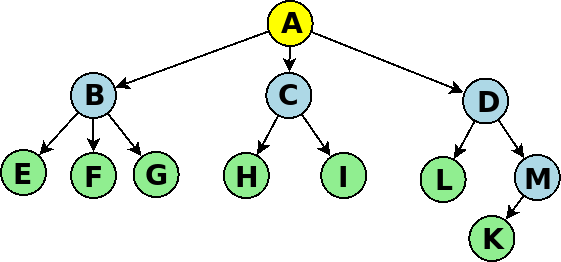
\includegraphics[width=0.7\linewidth]{img/tree_example}
	\label{fig:treeexample}
\end{figure}

Y para un mejor entendimiento asumiremos que los nodos hijos izquierdos serán todos menos el último hijo que será el derecho. De esta forma el nodo $B$ tiene dos hijos izquierdos ($E$,$F$) y un derecho ($G$).

\subsection{Recorrido en profundidad-primero}
\subsubsection{Preorden}

\emph{(\textbf{raíz}, izquierdo, derecho)}. Para recorrer un árbol no vacío en Preorden, hay que realizar
las siguientes operaciones recursivamente en cada nodo, comenzando con el nodo raíz:

\begin{itemize}
	\item Procesa la raíz
	\item Recorrer el subárbol izquierdo InOrden
	\item Recorrer el subárbol derecho InOrden
\end{itemize}

Si asumimos que el procesar la raiz es la impresión del valor almacenado en el nodo el recorrido en inorden en el árbol presentado de muestra anteriormente daría la siguiente secuencia o impresión de salida.

$$ A, B,E,F,G,C,H,I,D,L,M,K $$

\subsubsection{Inorden}

\emph{(izquierdo, \textbf{raíz}, derecho)}. El valor en un nodo no se procesa hasta que se procesen los valores en
su subárbol izquierdo.
Para recorrer un árbol no vacío en Inorden, hay que realizar las siguientes operaciones
recursivamente en cada nodo, comenzando con el nodo raíz:

\begin{itemize}
	\item Recorrer el subárbol izquierdo InOrden
	\item Procesa la raíz
	\item Recorrer el subárbol derecho InOrden
\end{itemize}

Si asumimos que el procesar la raiz es la impresión del valor almacenado en el nodo el recorrido en inorden en el árbol presentado de muestra anteriormente daría la siguiente secuencia o impresión de salida.

$$ E,F,B,G,H,C,I,A,L,D,K,M $$

\subsubsection{Postorden}

\emph{(izquierdo, derecho, \textbf{raíz})}. Para recorrer un árbol binario no vacío en Postorden, hay que realizar
las siguientes operaciones recursivamente en cada nodo, comenzando con el nodo raíz:

\begin{itemize}
	\item Recorrer el subárbol izquierdo InOrden
	\item Recorrer el subárbol derecho InOrden
	\item Procesa la raíz
\end{itemize}

Si asumimos que el procesar la raiz es la impresión del valor almacenado en el nodo el recorrido en inorden en el árbol presentado de muestra anteriormente daría la siguiente secuencia o impresión de salida.

$$ E,F,G,B,H,I,C,L,K,M,D,A $$

En general, la diferencia entre preorden, inorden y postorden es cuándo se recorre la raíz. En los tres, se recorre primero el sub-árbol izquierdo y luego el derecho. 

\begin{itemize}
	\item En preorden, la raíz se recorre antes que los recorridos de los subárboles izquierdo y derecho
	\item En inorden, la raíz se recorre entre los recorridos de los árboles izquierdo y derecho
	\item En postorden, la raíz se recorre después de los recorridos por el subárbol izquierdo y el derecho
\end{itemize}

Preorden (antes), inorden (en medio), postorden (después). 

\subsection{Recorrido en anchura-primero}
Los árboles también pueden ser recorridos en orden por nivel (de nivel en nivel), donde visitamos cada nodo en un nivel antes de ir a un nivel inferior. Esto también es llamado recorrido en anchura-primero o recorrido en anchura. Se etiquetan los nodos según su profundidad
(nivel). Se recorren ordenados de menor a mayor nivel, a igualdad de nivel
se recorren de izquierda a derecha.

Si asumimos que el procesar la raiz es la impresión del valor almacenado en el nodo el recorrido en anchura-primero en el árbol presentado de muestra anteriormente daría la siguiente secuencia o impresión de salida.

$$ A, B, C, D, E, F, G, H, I, L, M, K $$
\section{Implementación}
La implementaciones de los recorridos va depender en gran medida del tipo de árbol y de como fue implementado por lo que a continuación se van a presentar ideas generales de la implementación de estos recorridos asumiendo que estamos trabajando con árboles binarios.

\subsection{Recorrido en profundidad-primero}

\subsubsection{Preorden}

\begin{lstlisting}[language=C++]
//Variante recursiva 
preorden(nodo)
   si nodo == nulo entonces retorna
   imprime nodo.valor
   preorden(nodo.izquierda)
   preorden(nodo.derecha)
   
//Variante iterativa
iterativePreorder(node)
   if (node = null)
      return
   s = empty stack
   s.push(node)
   while (not s.isEmpty())
      node = s.pop()
      visit(node)
      if (node.right != null)
         s.push(node.right)
      if (node.left != null)
         s.push(node.left)   
\end{lstlisting}

\subsubsection{Inorden}

\begin{lstlisting}[language=C++]
//Variante recursiva 
inorden(nodo)
   si nodo == nulo entonces retorna
   inorden(nodo.izquierda)
   imprime nodo.valor
   inorden(nodo.derecha)
   
//Variante iterativa
iterativeInorder(node)
   s = empty stack
   while (not s.isEmpty() or node != null)
      if (node != null)
         s.push(node)
         node = node.left
      else
         node = s.pop()
         visit(node)
         node = node.right
\end{lstlisting}

\subsubsection{Postorden}

\begin{lstlisting}[language=C++]
//Variante recursiva 
postorden(nodo)
   si nodo == nulo entonces retorna
   postorden(nodo.izquierda)
   postorden(nodo.derecha)
   imprime nodo.valor
   
//Variante iterativa
iterativePostorder(node)
   s = empty stack
   lastNodeVisited = null
   while (not s.isEmpty() or node != null)
      if (node != null)
         s.push(node)
         node = node.left
      else
         peekNode = s.peek()
         if (peekNode.right != null and lastNodeVisited != peekNode.right)
            node = peekNode.right
         else
            visit(peekNode)
            lastNodeVisited = s.pop()
\end{lstlisting}

\subsection{Recorrido en anchura-primero}

También está el pseudocódigo para un simple recorrido en orden por nivel basado en cola.

\begin{lstlisting}[language=C++]
orden_por_nivel(raiz)
   cola = nueva cola
   cola.encola(raiz)
   mientras not cola.vacia hacer
      nodo = cola.desencola()
      visita(nodo)
      si nodo.izquierdo != null entonces
         cola.encola(nodo.izquierdo)
      si nodo.derecho != null entonces
         cola.encola(nodo.derecha)
\end{lstlisting}
\section{Aplicaciones}
Es particularmente común usar un recorrido inorden en un árbol binario de búsqueda porque éste retornará valores en el orden del conjunto subyacente, de acuerdo al comparador que configura el árbol de búsqueda binaria (de aquí el nombre).

Para ver porqué éste es el caso, note que si n es un nodo en un árbol binario de búsqueda, entonces todo n en el subárbol izquierdo es menor que n, y todo n en el subárbol derecho es mayor o igual a n. Por lo tanto, si visitamos el subárbol izquierdo en orden, usando una llamada recursiva, y entonces visitamos a n, y después visitamos el subárbol derecho en orden, nosotros hemos visitado completamente el subárbol con raíz en n en orden. Podemos asumir que las llamadas recurrentes visitan correctamente los subárboles en orden usando el principio matemático de inducción estructural. Similarmente, el recorrer en inorden reverso da los valores por orden decreciente. 

Recorriendo un árbol en preorden mientras se está insertando los valores en un nuevo árbol es una manera común de hacer una copia completa de un árbol binario de búsqueda.

También se pueden usar los recorridos preorden para conseguir una expresión prefijo 
(notación polaca) de árboles de expresión: recorra el árbol de expresión en 
preorden. Para calcular el valor de tal expresión: explore de derecha a izquierda, 
poniendo los elementos en un stack. Cada vez que se encuentre un operador, se 
sustituyen los dos símbolos superiores del stack por el resultado de aplicar al 
operador a esos elementos. Por ejemplo, la expresión * + 2 3 4, que en la notación 
de infijo es (2 + 3) * 4.
\section{Complejidad}
La complejidad tanto espacial como temporal de todos los recorridos es O($N$) donde $N$ es la cantidad de nodos que posee el árbol. Pero ten cuidado con las implementaciones recursivas y un árbol demasiado grande para ese caso analiza si se puede utilizar una implementación iterativa.
\section{Ejercicios}
A continuación una lista de ejercicios que se pueden resolver utilizando el contenido abordado en la guía:

\begin{itemize}
	\item \href{https://dmoj.uclv.edu.cu/problem/obilazak}{DMOJ - Visita a Sydney}
	\item \href{https://dmoj.uclv.edu.cu/problem/coldwat}{DMOJ - Agua Fría Clara}
\end{itemize}

\end{document}